\documentclass[12pt,a4paper]{book}

% Uporabljeni paketi
\usepackage[utf8]{inputenc}
\usepackage{cmap}
\usepackage{float}
\usepackage{type1ec}
\usepackage[T1]{fontenc}
\usepackage{fancyhdr}
\usepackage{graphicx,epsfig}
\usepackage[slovene]{babel}
\usepackage{tikz}
\usepackage{csquotes}
\usepackage[
  backend=biber,
  style=numeric,
  sorting=none,
]{biblatex}
\usepackage{hyperref}
\addbibresource{literatura.bib}
\usepackage{longtable}
\usepackage{geometry}
\usepackage{array}
\geometry{a4paper, margin=1in}

% Nastavitev glave in repa strani
\pagestyle{fancy}
\fancyhead{}
\renewcommand{\chaptermark}[1]{\markboth{\textsf{Poglavje \thechapter:\ #1}}{}}
\renewcommand{\sectionmark}[1]{\markright{\textsf{\thesection\  #1}}{}}
\fancyhead[RE]{\leftmark}
\fancyhead[LO]{\rightmark}
\fancyhead[LE,RO]{\thepage}
\fancyfoot{}
\renewcommand{\headrulewidth}{0.0pt}
\renewcommand{\footrulewidth}{0.0pt}

\newcommand{\gnuplot}{\textbf{gnuplot}}
\newcommand{\pgfname}{\textsc{pgf}}
\newcommand{\tikzname}{Ti\emph{k}Z}

\begin{document}
\thispagestyle{empty}
\begin{center}
{\large 
UNIVERZA V LJUBLJANI\\
FAKULTETA ZA RAČUNALNIŠTVO IN INFORMATIKO\\
}

\vspace{3cm}
{\LARGE Svit Spindler}\\

\vspace{2cm}
\textsc{\textbf{\LARGE
Hiter inženiring pri razvoju programske opreme\\ 
}}

\vspace{2cm}
{ DIPLOMSKO DELO}\\
{ NA UNIVERZITETNEM ŠTUDIJU\\
}

\vspace{2cm} 
{\Large Mentor: izr. prof. dr. Dejan Lavbič}

\vfill
{\Large Ljubljana, 2024}
\end{center}

\newpage

%********************************************

% stran 3 med uvodnimi listi
\thispagestyle{empty}

Namesto te strani {\bf vstavite} original izdane teme diplomskega dela s podpisom mentorja in dekana ter \v zigom fakultete, ki ga diplomant
dvigne v študent\-skem referatu,  preden odda izdelek v vezavo!

\newpage

\newpage

\ \thispagestyle{empty}

\newpage

%********************************************

% stran 2 med uvodnimi listi
\thispagestyle{empty}

\vspace*{5cm}
{\small \noindent
To diplomsko delo je ponujeno pod licenco \textit{Creative Commons Priznanje avtorstva-Deljenje pod enakimi pogoji 2.5 Slovenija}
ali (po želji) novejšo različico.
To pomeni, da se tako besedilo, slike, grafi in druge sestavine dela kot tudi rezultati diplomskega dela lahko prosto distribuirajo,
reproducirajo, uporabljajo, dajejo v najem, priobčujejo javnosti in predelujejo, pod pogojem, da se jasno in vidno navede avtorja in naslov tega
dela in da se v primeru spremembe, preoblikovanja ali uporabe tega dela v svojem delu, lahko distribuira predelava le pod
licenco, ki je enaka tej.
Podrobnosti licence so dostopne na spletni strani \url{http://creativecommons.si/} ali na Inštitutu za
intelektualno lastnino, Streliška 1, 1000 Ljubljana.

\begin{center}% 0.66 / 0.89 = 0.741573033707865

\end{center}
}

\vspace*{1.5cm}
{\small \noindent
Izvorna koda diplomskega dela, njenih rezultatov in v ta namen razvite programske opreme je ponujena pod GNU General Public License,
različica 3 ali (po želji) novejšo različico. To pomeni, da se lahko prosto uporablja, distribuira in/ali predeluje pod njenimi pogoji.
Podrobnosti licence so dostopne na spletni strani \url{http://www.gnu.org/licenses/}.
}

\begin{center} 
\ \\ \vfill
{\em
Besedilo je oblikovano z urejevalnikom besedil \LaTeX. \\ Slike so izdelane s pomočjo jezika \pgfname/\tikzname. \\ Grafi so narisani
s pomočjo programa \gnuplot.}
\end{center}

\newpage

\ \thispagestyle{empty}

\newpage

%********************************************

% stran 3 med uvodnimi listi
\thispagestyle{empty}

Namesto te strani {\bf vstavite} original izdane teme diplomskega dela s podpisom mentorja in dekana ter \v zigom fakultete, ki ga diplomant
dvigne v študent\-skem referatu,  preden odda izdelek v vezavo!

\newpage

%********************************************

% stran 4 med uvodnimi listi je prazna 
\ \thispagestyle{empty}

\newpage

%********************************************

% stran 5 med uvodnimi listi

\thispagestyle{empty}

\vspace{1cm}
\begin{center} 
{\Large \textbf{IZJAVA O AVTORSTVU}}
\end{center}

\begin{center} 
{\Large diplomskega dela}
\end{center}

\vspace{1cm}
Spodaj podpisani/-a \hspace{0.5cm} Ime Priimek,

\vspace{0.5cm}
z vpisno številko \hspace{0.5cm} xxxxxxx,

\vspace{1cm}
sem avtor/-ica diplomskega dela z naslovom:
   
\vspace{0.5cm}
Naslov diplomskega dela

\vspace{1.5cm}
S svojim podpisom zagotavljam, da:
\begin{itemize}
    \item sem diplomsko delo izdelal/-a samostojno pod mentorstvom prof. [doc.] dr. Ime Priimek in somentorstvom prof. [doc.] dr. Ime Priimek
    \item so elektronska oblika diplomskega dela, naslov (slov., angl.), povzetek (slov., angl.) ter ključne besede (slov., angl.) identični s tiskano obliko diplomskega dela
    \item soglašam z javno objavo elektronske oblike diplomskega dela v zbirki ''Dela FRI''.
\end{itemize}

\vspace{1cm}
V Ljubljani, dne xx.xx.20xx \hspace{1cm} Podpis avtorja/-ice:

\newpage 

%********************************************

% stran 6 med uvodnimi listi je prazna pri dvostranskem tiskanju
\ \thispagestyle{empty}

\newpage
\ \thispagestyle{empty}

%********************************************

% stran 7 med uvodnimi listi

\chapter*{Zahvala}

\thispagestyle{empty}

Na tem mestu se diplomant zahvali vsem, ki so kakorkoli pripomogli k uspešni izvedbi diplomskega dela.
\\**Zahvala podjetju Digital School D.O.O, za pomoč pri analizi učenja otrok z uporabo umetne inteligence. **


\newpage

%********************************************

% stran 8 med uvodnimi listi je prazna pri dvostranskem tiskanju
\ \thispagestyle{empty}

\newpage

%********************************************

\renewcommand\thepage{} 
\tableofcontents 
\renewcommand\thepage{\arabic{page}}

\thispagestyle{empty}


%********************************************

\chapter*{Seznam uporabljenih kratic in simbolov}

\thispagestyle{empty}

Seznam uporabljenih kratic in simbolov, ki morajo biti enotni v celotnem delu, ne glede na označevanje v uporabljenih virih.

\begin{table}[h!]
    \centering
    \begin{tabular}{|l|l|}
        \hline
        UI & umetna inteligenca \\
        \hline
        PNJ & procesiranje naravnih jezikov \\
        \hline
        GCC & GitHub Copilot Chat \\
        \hline
        IDE & integrirano razvojno okolje \\
        \hline
    \end{tabular}
    \caption{Seznam kratic in njihovih pomenov}
    \label{tab:abbreviations}
\end{table}

%\cleardoublepage

\clearpage{\pagestyle{empty}\cleardoublepage}

%********************************************
%zacno se glavni listi, ki so numerirani z arabskimi stevilkami

\setcounter{page}{1}
\pagenumbering{arabic}

\chapter*{Povzetek}
\addcontentsline{toc}{chapter}{Povzetek}

Povzetek naj posreduje bralcu kratko vsebino dela. Zajema naj namen dela, področje, na katerega se delo nanaša,
uporabljene metode, poglavitne rezultate dela, zaključke in priporočila. 
Povzetek naj ne obsega več kot eno stran, obi\v cajno ima le 200 do 300 besed. Napiše se povsem na koncu,
ko je že jasna vsebina vseh ostalih poglavij.

Ta dokument vsebuje navodilo za izdelavo diplomskega dela v obliki in strukturi, ki je v teh navodilih predpisan za
pisanje diplomskih nalog. Struktura dokumenta je namenjena obojestranskemu tiskanju, kjer se novo poglavje vedno za\v cne na lihi strani.
V dejanski diplomi poglavja in podpogla\-vja  obi\v cajno niso tako kratka kot v teh navodilih.

Za oblikovanje tega dokumenta je bil uporabljen sistem \LaTeX.
Ve\v c o \LaTeX-u lahko izve\v s na spletni strani \texttt{http://www.ctan.org/}.
Kandidati, ki bodo svoje diplomsko delo oblikovali s pomo\v cjo
\LaTeX-a, lahko izvorno kodo tega dokumenta neposredno uporabijo kot vzorec za pisanje svoje diplomske naloge.

\vspace{1.3cm}
\noindent
{\large \bf Ključne besede:}

\vspace{0.5cm}
\noindent
diploma, mentor, zagovor, podaljšanje, pisanje, struktura


\chapter*{Abstract}

\addcontentsline{toc}{chapter}{Abstract}

Povzetek naj bo napisan v angleškem jeziku.

\vspace{1.3cm}
\noindent
{\large \bf Key words:}

\vspace{0.5cm}
\noindent
Ključne besede v angleškem jeziku.


%********************************************

\chapter{Uvod}

Orodja za dopolnjevanje in generiranje kode so pri programiranju postala zelo popularna, saj omogočajo hitrejše in učinkovitejše reševanje problemov. Orodja za generiranje kode s pomočjo umetne inteligence, kot so GitHub Copilot, Amazon CodeWhisperer in ChatGPT podjetja OpenAI se uporabljajo tako med začetniki kot tudi med izkušenimi programerji. Ta orodja omogočajo generiranje kode na podlagi pozivov v naravnem jeziku ali delnih vnosov kode, kar bistveno poenostavi proces programiranja.

Namen te študije je preučiti prednosti in slabosti najpopularnejših orodij za umetno inteligenco (UI) ter raziskati, kako omenjena orodja vplivajo na proces učenja in programiranja pri začetnih programerjih s preučevanjem hitrosti in kvalitete kode na različnih programerskih problemih v jeziku Python. V dobi, ko postaja UI vedno bolj dostopna in popularna, je ključnega pomena raziskati, ali lahko UI pospeši proces učenja in izboljša razumevanje programerskih konceptov.  

V naslednjih poglavjih bomo pregledali razvoj programske kode in vlogo strojnega učenja ter naprednih jezikovnih modelov pri avtomatizaciji tega procesa. Najprej bomo raziskali zgodovinski razvoj orodij za podporo razvijalcem in zgodnje uporabe strojnega učenja pri pridobivanju specifikacij in napovedovanju uporabniškega vnosa. Nato bomo obravnavali sodobne arhitekture globokega učenja, kot sta GPT-3 in GPT-4, ki omogočajo napredne funkcionalnosti avtomatskega dopolnjevanja in generiranja kode.



\chapter{Pregled področja}
Narava in kompleksnost programske opreme sta se v zadnjih 30 letih močno spremenili. V sedemdesetih letih 20. stoletja so aplikacije delovale na enem samem procesorju, proizvajale alfanumerične izhode in prejemale svoj vhod iz linearnega vira. Današnje aplikacije so veliko bolj zapletene; običajno imajo grafični uporabniški vmesnik in uporabljajo arhitekturo odjemalec-strežnik. Pogosto delujejo na dveh ali več procesorjih, pod različnimi operacijskimi sistemi in na geografsko porazdeljenih strojih. Redko katero področje v zgodovini se je  razvilo tako hitro kot razvoj programske opreme. Zato je nujno stalno potrebno izboljševati koncepte, strategije in prakse programskega inženiringa, da bi se izognili konfliktom in izboljšali proces razvoja programske opreme, da bi pravočasno in v okviru proračuna zagotovili kakovostno programsko opremo, ki jo je mogoče vzdrževati.
\cite{aggarwal2005software}
\section{Programski inženiring}
Programska oprema je postala ključna za napredek na skoraj vseh področjih človekovega delovanja. Programiranje samo ne zadostuje več za izdelavo velikih programov. Obstajajo resne težave pri kakovosti,stroških, pravočasnosti in vzdrževanju številnih izdelkov programske opreme.
Cilj programskega inženiringa je reševanje teh težav z izdelavo kakovostne programske opreme, ki je narejena pravočasno in v okviru proračuna. Da bi dosegli ta cilj, se moramo osredotočiti tako na kakovost izdelka kot tudi na procese, uporabljene za razvoj izdelka.
Na prvi konferenci o programskem inženiringu leta 1968 je Fritz Bauer 
definiral programski inženiring kot "Vzpostavitev in uporaba dobrih inženirskih principov za pridobitev ekonomično razvite programske opreme, ki je zanesljiva in učinkovito deluje na resničnih strojih". Stephen Schach je enako opredelil kot "Področje, katerega cilj je izdelava kakovostne programske opreme, ki je izdelana pravočasno, v okviru predvidenega proračuna in izpolnjuje zastavljene zahteve.". Obe definiciji sta priljubljeni in sprejemljivi za večino. Vendar pa se zaradi povečanja stroškov vzdrževanja programske opreme cilj zdaj premika k izdelavi kakovostne programske opreme, ki jo je mogoče vzdrževati, dostavljeno pravočasno, v okviru proračuna in prav tako izpolnjuje njene zahteve.
Kriza programske opreme nas spremlja že od leta 1970. Od takrat se je računalniška industrija z računalniško revolucijo in nedavno z omrežno revolucijo, ki jo je sprožila in/ali pospešila eksplozivna širitev interneta in v zadnjem času spleta, razvijala z bliskovito hitrostjo.
Računalniška industrija je zagotavljala eksponentno izboljšanje razmerja med ceno in zmogljivostjo, vendar se težave s programsko opremo niso zmanjševale. Programska oprema še vedno zamuja, presega proračun in je polna napak. Po zadnjem IBM-ovem poročilu je "31 \% projektov preklicanih, še preden so končani, 53 \% projektov presega oceno stroškov za povprečno 189 \%, na vsakih 100 projektov pa je 94 ponovnih zagonov".
\cite{aggarwal2005software}


Razvoj programske kode je proces, ki vključuje pretvorbo specifikacije problema v programsko implementirano rešitev. Zgodnja orodja za olajšanje postopka so uporabljala strojno učenje za podporo razvijalcev skozi vse faze razvoja programske opreme in so med drugimi vključevala pridobivanje programske specifikacije in napoved uporabnikovega vnosa.
Med zgodnjo opremo sodijo orodja za dopolnjevanje kode, ki so na voljo v večini urejevalnikov kode in ki izpišejo kontekstualno relevantne spremenljivke, metode, razrede in druge dele kode v obliki plavajočega menija. Razvijalci se lahko z raziskovanjem in izbiranjem v tem meniju izognejo pogostim slovničnim in logičnim napakam, zmanjšajo število pritiskov na tipke in raziskujejo nove API-je namesto da porabljajo čas in napor za iskanje dokumentacije. Nekatera znana orodja za dopolnjevanje kode vključujejo IntelliSense v Visual Studio Code in vgrajeno dopolnjevanje kode v orodjih JetBrains IDE2. 
Čeprav lahko ta orodja izpisujejo odlomke kode, se bistveno razlikujejo od generatorjev kode.
Z današnjimi napredki na področjih globokega učenja in procesiranja naravnega jezika so se razvili napredni modeli za pomoč pri kodiranju, ki omogočajo avtomatsko dopolnjevanje in reševanje problemov v kodi v realnem času.
Obstaja veliko poskusov samodejnega prevajanja specifikacij v računalniško kodo s pomočjo formalnih modelov za avtomatsko generiranje kode ali pa s pomočjo strojno naučenega procesiranja naravnega jezika. Arhitekture globokega učenja, ki se dobro prilegajo procesiranju naravnega jezika, so omogočile razvoj modelom ko sta GPT-2 in GPT-3. Ti modeli lahko izvajajo jezikovne naloge, kot sta prevajanje in odgovarjanje na vprašanja iz nabora podatkov pogovornega naziva za odgovarjanje na vprašanja (angl. CoQA). Po prilagajanju glede na specializiran nabor podatkov lahko modeli opravljajo naloge, kot so dopolnjevanje kode in načrtovanje strojne opreme.  Najsodobnejši modeli imajo na milijarde parametrov, ki jih je mogoče natrenirati, in so učeni na več milijonih programskih repozitorijev. V tem delu se bomo osredotočili na modele ChatGPT, GitHub Copilot in Amazon Codewhisperer ter jih medsebojno primerjali.
V naslednjem poglavju bomo najprej pregledali obstoječo literaturo povezano z uporabo UI s poudarkom na hitrem inženiringu in razvoju programske opreme s pomočjo UI. 
\cite{zhang2003machine}
\section{Sorodna literatura}

\cite{app13095783}

Med že objavljenimi deli so bile raziskane priložnosti in izzivi uporabe ChatGPT v izobraževanju. Ugotovili so, da ChatGPT ponuja velike prednosti, kot so omogočanje personaliziranega učenja in zagotavljanje takojšnjih povratnih informacij, vendar prinaša tudi izzive, vključno z možnostjo prekomerne odvisnosti od UI in potrebo po splošni digitalni pismenosti med študenti.
Uporaba modelov, ki temeljijo na UI, kot je ChatGPT, v računalniškem programiranju je obširno raziskana. Ti modeli so uspešni pri nalogah, kot so dopolnitve kode, povzemanje, dokončanje, popravljanje, razvrščanje in generiranje kode. Na primer, AlphaCode, napreden jezikovni model, je pokazal znatne zmožnosti pri različnih programerskih nalogah, kar poudarja potencial ChatGPT pri pomoči pri izobraževanju programiranja. \cite{rudolph2023war}
\newline
V delu \textcite{MORADIDAKHEL2023111734} je raziskano programiranje s programom GitHub Copilot, kjer se primerja kvaliteta in pravilnost rešitev, ki jih le ta ponuja.
Sorodno delo je tudi \textcite{yetistiren2023evaluating}, kjer je narejena primerjava GitHub Copilot, Amazon CodeWhisperer in ChatGPT. V delu se omenjena orodja primerja, ter raziskuje pravilnost, kvaliteta, varnost in zanesljivost generirane kode za vsako orodje.
Veliko del je bilo narejenih z namenom preučevanja kvalitete in pravilnosti kode, ki jo orodja UI generirajo. Pri teh študijah se je potrebno zavedati, da se orodja UI stalno in zelo hitro razvijajo in lahko rezultati meril uspešnosti, ki so bili pridobljeni v preteklosti, ne držijo več za novejše verzije orodij.
Pri iskanju sorodne literature je bilo najdenih veliko del, ki preučujejo generirano kodo orodij UI. Ni pa bila še narejena študija, ki bi primerjala hitrost in pravilnost programiranja začetnikov ob souporabi ChatGPT napram njihovi kakovosti programiranja brez orodij. V naslednjih poglavjih bomo preučili razvoj orodij UI ter najpopularnejše predstavnike tudi primerjali.


\chapter{Hiter inženiring}

Hiter inženiring je razmeroma nova tehnika na področju obdelave naravnega jezika, ki zajema načrtovanje in optimizacijo pozivov, ki se uporabljajo za vnos informacij v modele UI, da bi izboljšali njihovo učinkovitost pri določenih nalogah. \cite{wang2024prompt} Gre za prakso učinkovitega sodelovanja s sistemi UI za optimizacijo njihovih koristi. Z nedavnim napredkom velikih jezikovnih modelov se je hitro inženirstvo izkazalo za pomembno in učinkovito na različnih področjih, vse od programiranja in učenja, do področja financ in zdravstva.
\cite{info:doi/10.2196/50638}

\section{Veliki jezikovni modeli}
Veliki jezikovni modeli so vrsta umetne inteligence, zasnovana za razumevanje in ustvarjanje besedila, ki je blizu ljudem. Treniranje temelji na vnaprej naučenih vzorcih z obsežnim usposabljanjem na veliki količini podatkov, kot so spletne strani, knjige in članki. S pomočjo podatkov lahko model prepozna statistične vzorce in strukture človeškega jezika, kar omogoča, da se nauči slovnice, sintakse in semantične odnose v jeziku. Po končanem učenju se model navadno usmeri in prilagodi za določeno domeno ali nalogo, kot je na primer prevajanje, generiranje besedila, prepoznavanje slik, ipd.
\cite{10.1145/3520312.3534862}
V zadnjih letih je prišlo do velikega napredka na področju procesiranja naravnih jezikov (PNJ) predvsem z razvojem arhitekture transformatorjev in mehanizma pozornosti.
Transformator je arhitektura globokega učenja, ki jo je razvil Google in temelji na mehanizmu večglave pozornosti, predstavljenem v članku "Attention Is All You Need" iz leta 2017.  \cite{datacamp_attention_2024} 
Besedilo se pretvori v numerične reprezentacije, imenovane žetoni, vsak žeton pa se s pomočjo tabele za vstavljanje besed pretvori v vektor. Na vsaki plasti se nato vsak žeton kontekstualizira z drugimi žetoni prek vzporednega mehanizma večglave pozornosti, ki omogoča, da se signal za ključne žetone okrepi, manj pomembni žetoni pa se zmanjšajo. To modelu omogoča boljše razumevanje odnosov med besedami v stavku, ne glede na njihov položaj.
Rekurentne enote so komponente v nekaterih nevronskih mrežah, ki si zapomnijo prejšnje informacije, da lahko pri obdelavi novega podatka upoštevajo kontekst. Vendar pa zaradi tega potrebujejo več časa za treniranje, ker morajo vsakič obdelati informacije korak za korakom.
Prednost transformatorjev je, da nimajo rekurentnih enot, kar jim omogoča, da obdelujejo podatke hitreje in bolj učinkovito. Poleg transformatorjev je pomembne spremembe prinesel tudi mehanizem pozornosti.
\cite{NIPS2017_3f5ee243}

Mehanizem pozornosti za razliko od tradicionalnih metod, ki besede obravnavajo ločeno, vsaki besedi dodeli uteži glede na njeno pomembnost za trenutno nalogo. To modelu omogoča, da zajame odvisnosti dolgega dosega, hkrati analizira lokalne in globalne kontekste ter razrešuje dvoumnosti s pozornostjo do informativnih delov stavka. Razvoj tega mehanizma je doprinesel k razvoju velikih jezikovnih modelov.
\cite{datacamp_attention_2024}
\cite{KASNECI2023102274}

Druga pomembna novost je uporaba učenja vnaprej, pri katerem se jezikovni model najprej uči na velikem naboru podatkov, nato pa se prilagodi določeni nalogi. To se je izkazalo za učinkovito tehniko za izboljšanje učinkovitosti pri številnih jezikovnih nalogah.
Nedavni napredek vključuje tudi razvoj najpopularnejšega modela ChatGPT, ki je bil učen na veliko večji zbirki podatkov, tj. besedilih iz zelo velikega spletnega korpusa, in je pokazal vrhunsko uspešnost pri številnih nalogah v naravnem jeziku, od prevajanja do odgovarjanja na vprašanja, pisanja koherentnih esejev in računalniških programov.
\cite{KASNECI2023102274}

Čeprav je razvoj velikih jezikovnih modelov zelo napredoval, je še vedno veliko omejitev, ki jih je treba odpraviti. Ena glavnih omejitev je pomanjkanje razlage odločitev, saj je težko razumeti razloge za napovedi modela. Obstajajo tudi etični pomisleki, kot so pomisleki glede pristranskosti in vpliva teh modelov, npr. na zaposlovanje, tveganje zlorabe in neustrezne ali neetične uporabe, izguba integritete in številni drugi. Na splošno bodo veliki jezikovni modeli še naprej premikali meje mogočega pri obdelavi naravnega jezika. Vendar je treba opraviti še veliko dela v smeri obravnavanja njihovih omejitev in s tem povezanih etičnih vidikov.

Jezikovni modeli dodeljujejo verjetnosti zaporedjem žetonov in se pogosto uporabljajo za besedila v naravnem jeziku. V zadnjem času so jezikovni modeli pokazali učinkovitost tudi pri modeliranju izvorne kode, napisane v programskih jezikih. Ti modeli se izkažejo pri nalogah, kot sta dopolnjevanje kode ter sintetizacija kode iz opisov v naravnem jeziku. 
Trenutni najsodobnejši veliki jezikovni modeli za kodo so pokazali pomemben napredek pri pomoči pri programiranju z asistenco umetne inteligence. Najbolj izstopa eden največjih modelov, Codex, ki se kot orodje GitHub Copilot uporablja kot pomočnik za razvijalce znotraj IDE, ki samodejno ustvarja kodo na podlagi uporabnikovega vnosa. V naslednjih poglavjih bomo analizirali model Codex ter orodje GitHub Copilot, ChatGPT ter orodje Amazon CodeWhisperer.

\cite{KASNECI2023102274}
\cite{vaswani2023attention}

\section{ChatGPT}

ChatGPT je jezikovni model, ki ga je 30. novembra 2022 objavila organizacija OpenAI in je na voljo od 1. februarja 2023. \cite{openai_codex}
ChatGPT uporablja napredne algoritme strojnega učenja za ustvarjanje človeku podobnih odgovorov. Treniran je na obsežni količini tekstovnih besedil iz interneta. Glavni namen uporabe jezikovnega modela je imitiranje človeškega pogovora, kljub temu pa je zelo vsestranski in lahko opravlja številne naloge, kot so kodiranje in odpravljanje hroščev v programski opremi, iskanje odgovorov na izpitna
vprašanja, sestavljanje pesniških del in glasbenih besedil ter mnogo drugih nalog. ChatGPT je bil posebej prilagojen na podlagi modela iz serije GPT-3.59, ki je v začetku leta 2022 zaključil svoj proces usposabljanja z uporabo nadzorovanega učenja, kot tudi učenja z okrepitvijo. Poleg tega organizacija OpenAI še naprej zbira povratne informacije iz pogovorov z ChatGPT, da bi izboljšali in izpopolnili njegovo delovanje.
Omembe vredno je tudi, da je ChatGPT postal najhitreje rastoča aplikacija v zgodovini
glede na študijo švicarske banke Union 'Bank of Switzerland'. Januarja 2023 je ChatGPT dnevno obiskalo 13 milijonov unikatnih obiskovalcev, kar je več kot dvakrat toliko kot v istem letu decembra, kot je pokazala študija. Poročilo navaja tudi, da je v prvih dveh mesecih ChatGPT dosegel mesečno bazo uporabnikov 100 milijonov. \cite{yetistiren2023evaluating}

Napredek na področju UI, zlasti velikih jezikovnih modelov, je močno vplival na številna področja, vključno z izobraževanjem in razvojem programske opreme. ChatGPT je postalo pomembno orodje tako v izobraževalnih okoljih kot tudi v praktičnih programerskih aplikacijah. To poglavje obravnava vlogo ChatGPT v hitrem inženiringu in razvoju programske opreme, ocenjuje njegove prednosti, izzive in prihodnje vplive.
Hiter inženiring vključuje oblikovanje vhodov za modele UI, da bi dosegli želene odzive. Kot model UI, usposobljen na obsežnih podatkovnih zbirkah, je ChatGPT pokazal izjemno sposobnost interpretacije in generiranja besedil, podobnih človeškim, na podlagi različnih pozivov. Ta sposobnost je neprecenljiva v izobraževalnih okoljih, kjer lahko pomaga pri ustvarjanju interaktivnih učnih okolij, zagotavljanju takojšnjih povratnih informacij in generiranju učne vsebine. Na primer, ChatGPT lahko pomaga študentom pri razlagi zapletenih konceptov na enostavnejši način, s čimer izboljša njihovo učno izkušnjo.
Na področju razvoja programske opreme ChatGPT nudi veliko podporo pri generiranju kode, odpravljanju napak in optimizaciji. Orodja, kot so GitHub Copilot in Amazon CodeWhisperer, ki jih poganjajo modeli UI, podobni ChatGPT, pomagajo razvijalcem pri generiranju delov kode na podlagi opisov v naravnem jeziku. Ta funkcionalnost ne samo pospešuje proces kodiranja, temveč tudi pomaga začetnikom pri razumevanju strukture in sintakse kode.
Integracija ChatGPT v izobraževalne sisteme predstavlja številne priložnosti in izzive. Pozitivno je, da ChatGPT lahko demokratizira dostop do izobraževanja, saj zagotavlja prilagojeno mentorstvo in pomoč študentom po vsem svetu. Omogoča interaktivne učne izkušnje in pomaga pri razumevanju zapletenih predmetov, kot je programiranje. Raziskave so pokazale, da študenti, ki uporabljajo ChatGPT za programerske naloge in reševanje problemov, dosegajo boljše rezultate in razumevanje.

Vendar pa uporaba ChatGPT prinaša tudi tveganja, vključno z morebitnim prekomernim zanašanjem na UI za reševanje problemov, kar lahko ovira razvoj kritičnega mišljenja. Poleg tega je potrebno nenehno preverjanje natančnosti in zanesljivosti vsebine, ki jo generira UI, da bi preprečili širjenje napačnih informacij.
\cite{app13095783}
\section{GitHub Copilot}

GitHub Copilot je napredno orodje za generiranje kode v realnem času, ki se uporablja znotraj različnih integriranih razvojnih okolij (angl. IDE), kot so Visual Studio Code, Neovim, okolja JetBrains in GitHub Codespaces. GitHub Copilot neprekinjeno zbira uporabniške vnose kode in pošilja izseke v osnovni model OpenAI Codex podjetja OpenAI. Copilot generira kodo in predstavi rezultate modela OpenAI Codex tako, da predlagano generirano kodo prilagodi trenutni napisani kodi programerja znotraj IDE. Copilot je zmožen generirati kodo na podlagi opisa programskega problema v naravnem jeziku, kar omogoča reševanje nalog z generiranjem ustrezne kode. Poleg tega zna Codex kodo razložiti, jo prevesti med programskimi jeziki, napisati dokumentacijo, ter poiskati in popraviti napake v kodi.
Pomembna razširitev Copilota je GitHub Copilot Chat (GCC) , ki je bil objavljen 29. 12. 2023 in temelji na modelu GPT-4 podjetja OpenAI namesto modela Codex. Codex je starejši model, ki izhaja iz GPT-3 modela, ki je bil narejen v sodelovanju s podjetjem Github posebej za generiranje kode. GPT-4 ni razvit posebej za kodiranje, vendar je močno izboljšan model v primerjavi z modelom GPT-3.
\cite{Sundqvist1866649}
GCC znotraj IDE urejevalnika doda pogovorno okno, kjer lahko razvijalec v poljubnem naravnem jeziku postavlja vprašanja, zahteva razlago ali popravke kode, ter celo generiranje dokumentacije ali testov, brez da bi zapustil IDE. Poleg poziva, ki ga podamo v pogovorno okno GCC upošteva tudi kontekst trenutno odprte datoteke urejevalnika, dodatno pa lahko v kontekst pogovora v urejevalniku odprtega projekta referenciramo poljubne datoteke, ki se nanašajo na naše vprašanje, da dobimo bolj natančen odgovor.
\cite{github_copilot_chat}
\newline
Copilot temelji na družini modelov OpenAI Codex. Modeli Codex kot osnovo vzamejo model GPT-3, ki ga nato prilagodijo na podlagi kode iz GitHuba. Njegov način tokenizacije je skoraj identičen z GPT-3, uporablja kodiranje parov bajtov za pretvorbo izvornega besedila v zaporedje žetonov, vendar je bil besedni zaklad GPT-3 razširjen z dodajanem namenskih žetonov za bele prostore (tj. žeton za dva presledka, žeton za tri presledke, vse do 25 presledkov). To tokenizerju omogoča učinkoviteje kodiranje izvorne kode. (ki ima veliko belih presledkov) Pomembna lastnost, ki sta jo Codex in Copilot podedovala od GPT-3, je, da ob pozivu ustvarita najverjetnejši odgovor za poziv na podlagi tega, kar je bilo pridobljeno iz izkušenj, pridobljenih pri usposabljanju. V kontekstu generiranja kode to pomeni, da model ne bo nujno ustvaril najboljše kode (po kateri koli izbrani metriki - zmogljivost, varnost itd.), temveč tisto, ki se najbolje ujema s predhodno in naučeno kodo. Posledično na kakovost generirane kode močno vlivajo semantično nepomembne lastnosti poziva. \cite{9833571}
\cite{10.1145/3520312.3534862}



\section{Amazon CodeWhisperer}
Amazon CodeWhisperer izboljša produktivnost razvijalcev z generiranjem priporočil za kodo na podlagi komentarjev razvijalcev v angleščini in predhodne kode v IDE. AWS je napovedal Amazon CodeWhisperer 23. junija 2022. Predlogi kode, ki jih ponuja temeljijo na modelih strojnega učenja, ki so bili naučeni na različnih Amazonovih podatkovnih virih ter z odprtokodnimi repozitoriji. Ko
razvijalci napišejo komentar v urejevalniku kode v svojem IDE, CodeWhisperer samodejno pregleda komentar in določi najprimernejše storitve v oblaku in javne knjižnice. Nato bo neposredno v urejevalniku kode vrnil odlomek kode. CodeWhisperer razvijalcem dodatno poenostavi uporabo storitev AWS, saj ponuja predloge za AWS API kodo v storitvah, kot je Amazon Elastic Compute Cloud (EC2), AWS Lambda in Amazon Simple Storage Service (S3). CodeWhisperer podpira več IDE, vključno z JetBrains, Visual Studio Code, AWS Cloud9 ali konzolo AWS Lambda kot del nabora orodij AWS IDE. Trenutno podpira Javo, JavaScript, Python, C\# in Typescript. Kot dodatno funkcijo ima CodeWhisperer sledilnik referenc, ki zazna priporočila za kodo podobne določenim podatkom za usposabljanje CodeWhispererja in ta priporočila posreduje razvijalcem. CodeWhisperer zna kodo tudi pregledati ter opredeliti varnostna tveganja.

\section{Ugotovitve in primerjava}

\begin{table}[H]
\centering
\caption{Primerjava orodij ChatGPT, GitHub Copilot in Amazon CodeWhisperer}
\begin{tabular}{|>{\raggedright\arraybackslash}p{3cm}|>{\raggedright\arraybackslash}p{4cm}|>{\raggedright\arraybackslash}p{4cm}|>{\raggedright\arraybackslash}p{4cm}|}
\hline
\textbf{Lastnost}               & \textbf{ChatGPT}           & \textbf{GitHub Copilot}           & \textbf{Amazon CodeWhisperer}          
\\ \hline
Razvijalec              & OpenAI      & OpenAI-Microsoft                  & AWS            \\ \hline
Datum izdaje               & 30. 11. 2022        & 29. 10. 2021           & 23. 06. 2022       \\ \hline
Podpora integriranega razvojnega okolja           & Ni podpore          & Večina razvojnih okolij        & Pomembnejša razvojna okolja          \\ \hline
Razlaga predlagane kode       & Da                       & Da (omogoča GitHub Copilot Chat)                           & Ne                       \\ \hline
Navajanje sklicev na predloge                  & Ne                      & Ne                    & Da                      \\ \hline
Več predlogov za poziv                & Ne (možno z eksplicitnimi navodili za več predlogov)         & Da (do 10)                  & Da (do 5)               \\ \hline
Vir podatkov za usposabljanje             & GitHub repozitoriji, zbirka podatkov OpenAI Codex, online repozitoriji GitLab, Bitbucket in SourceForge                   & "Velike količine javno objavljene kode"                  & "...treniran na vseh jezikih iz javnih repozitorijev"                    \\ \hline
S katerimi jeziki deluje najboljše                        & Ni zapisano                  & C, C++, C\#, Go, Java, JavaScript, PHP, Python, Ruby, Scala in TypeScript              & C\#, Java, JavaScript, Python in TypeScript  \\ \hline
Cena               & osnovni model zastonj, plus 20\$ / mesec          & Zastonj za študente in učitelje, 10\$ / mesec za posameznike, 19\$ / mesec za profesionalne uporabnike                    &   Zastonj za posameznike, 19\$ / mesec za profesionalne uporabnike            \\ \hline
\end{tabular}
\label{tab:comparison}
\end{table}

Iz javno dostopnih podatkov ter testiranja zgoraj najpopularnejših predhodno omenjenih orodij smo naredili zgornjo tabelo, ki primerja modele ChatGPT, GitHub Copilot ter Amazon CodeWhisperer. Integracijo v razvojno okolje podpirata tako GitHub Copilot kot tudi Amazon CodeWhisperer, kjer GitHub Copilot ponuja bolj obširno izbiro razvojnih orodij. Razlago predlagane kode podpirata ChatGPT in GitHub Copilot Chat, sklice na predlagane rešitve pa ponuja le Amazon CodeWhisperer. Največje število predlogov za podan poziv ponuja Github Copilot, pri uporabi ChatGPT pa lahko to dosežemo z eksplicitnimi navodili. ChatGPT nima podanih informacij o najbolje podprtih programskih jezikih, GitHub Copilot in Amazon CodeWhisperer navajata podprte programske jezike, pri čemer lahko vidimo, da GitHub Copilot podpira več programskih jezikov kot Amazon CodeWhisperer. Pomembna razlika v modelih je tudi v ceni, saj nižja cena pripomore k različni dostopnosti širši množici uporabnikom, kar je eden izmed razlogov za popularnost ChatGPT-ja tudi v programiranju, kljub temu, da to ni njegov prvotni namen. Kljub temu, da je osnovni model zastonj, pa lahko plačamo 20\$ na mesec za napredni model, ki uporablja GPT-4. Amazon CodeWhisperer ima tudi ugoden cenovni načrt z možnostjo brezplačne uporabe za posameznike in ceno 19\$ mesec za profesionalne uporabnike. GitHub Copilot ponuja brezplačno uporabo le za učitelje in študente, ostali uporabniki plačujejo 10\$ / mesec ali pa 19\$ / mesec, če gre za profesionalne uporabnike.
\cite{github_copilot_chat}
\cite{openai_chatgpt}
\cite{saasworthy_codewhisperer}

\chapter{Metodologija}
Namen diplomskega dela je bil raziskati, kako hiter inženiring vpliva na proces razvoja programske opreme, s preučevanjem hitrosti in kvalitete kode pri uporabi orodij umetne inteligence. Najprimernejša metoda za pridobivanje teh podatkov je bil nadzorovan eksperiment na skupini mlajših otrok, ker omogoča natančen nadzor nad spremenljivkami ter izolirano vrednotenje reševanja programskih problemov. Ta metodologija minimizira vplive zunanjih spremenljivk, kar omogoča osredotočeno preučevanje zmožnosti in omejitev hitrega inženiringa pri razvoju programske opreme.

\section{Načrt}

\begin{figure}[H]
    \centering
    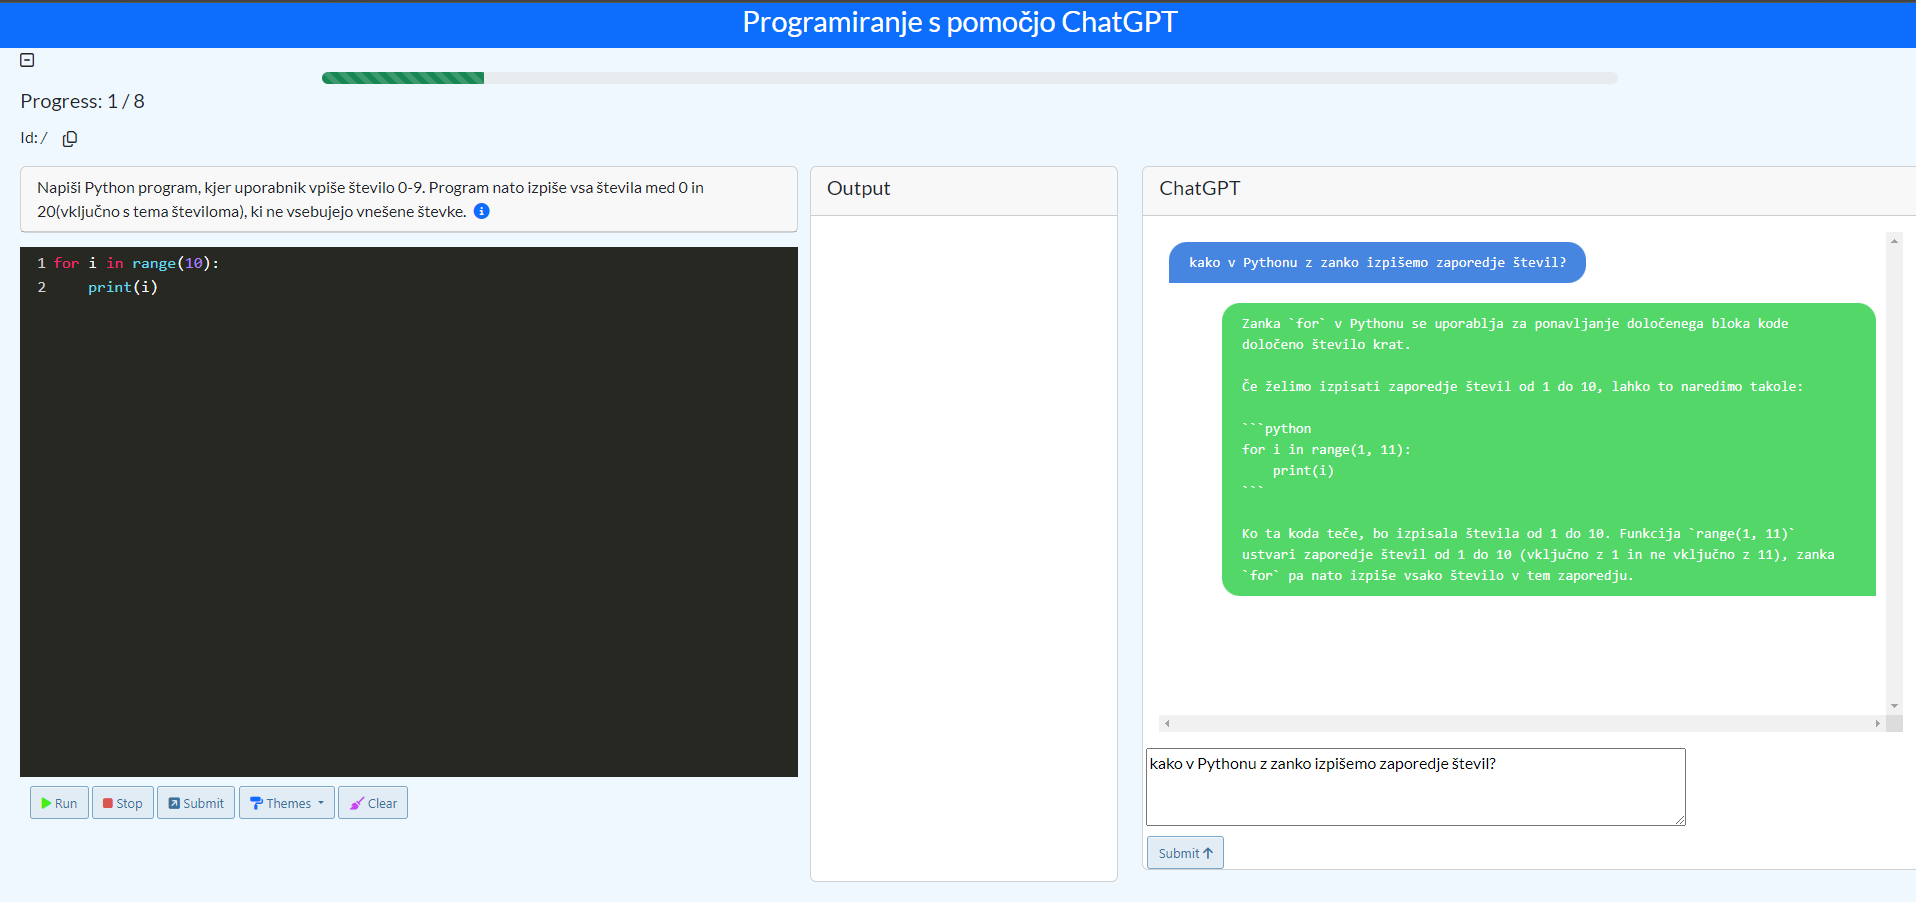
\includegraphics[width=1\linewidth]{spletna_stran.png}
    \caption{Spletna stran eksperimenta}
    \label{fig:enter-label}
\end{figure}


Za izvedbo eksperimenta smo izbrali več skupin mlajših otrok, ki se učijo programiranja v jeziku Python. Za namen eksperimenta je bila razvita preprosta spletna stran, ki je imela navodila za različne naloge, prostor za pisanje Python kode z označevanjem sintakse, prostor za izpis izhoda programa ter prostor za pogovor z uporabo ChatGPT-3.5. Namen strani je bil anonimizirano shranjevanje kode med eksperimentom, za namen kasnejšega preučevanja. Stran je kodo shranila ob vsakem kliku na gumb "Run" za izvajanje napisane kode ter na določen časovni interval. Shranjevalo se je napisano kodo, čas zapisa, število poskusov za trenutno nalogo ter če se je trenutna koda izvedla z napako. Eksperiment je trajal dve uri z vmesnih petnajst minutnim odmorom in je bil sestavljen iz osmih nalog. Vrstni red reševanja nalog je bil naključen brez možnosti vračanja na predhodne naloge, da bi zmanjšali prepisovanje. Za polovico nalog je bila uporaba chatGPT onemogočena, za lažjo analizo podatkov. Naloge so bile razdeljene v tri skupine težavnosti: lahke, srednje težke in težke. Težavnost naloge je bila dodeljena po pogovoru z ostalimi učitelji Pythona, glede na potrebno znanje in časovno zahtevnost naloge.

\begin{figure}[H]
    \centering
    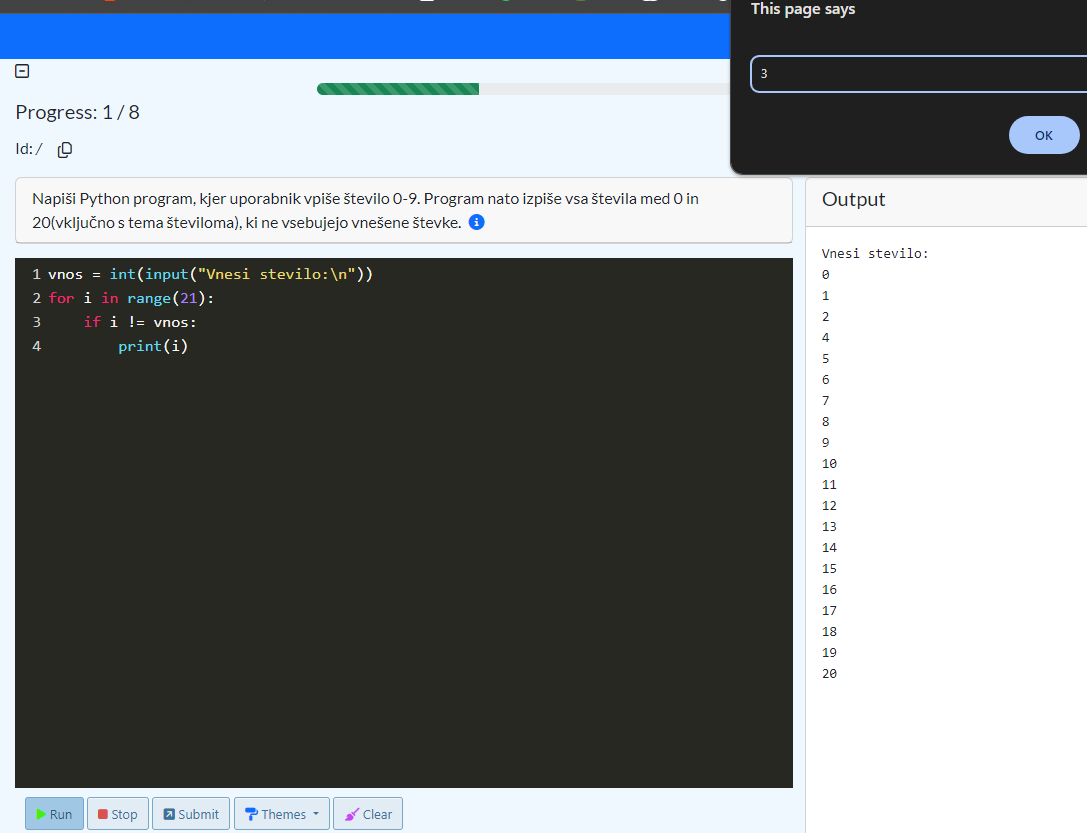
\includegraphics[width=1\linewidth]{naloga_primer.png}
    \caption{Primer naloge}
    \label{fig:enter-label}
\end{figure}
\section{Izvedba}
Eksperiment je bil izpeljan v štirih skupinah, ena izmed teh je bila v fizični obliki, ostale skupine pa so bile na daljavo. Skupaj je bilo veljavnih 32 podatkov. Eksperiment je potekal tako, da je bilo najprej predstavljena umetna inteligenca in hiter inženiring, ter najboljše prakse za uporabo ChatGPT za pomoč pri programiranju. Nato je bila rešena krajša anketa o predznanju programiranja ter o poznavanju ChatGPT-ja. Po tem so imeli dobro uro za samo reševanje nalog. Med samim eksperimentom se otrokom ni pomagalo, razen z interpretacijo navodil.
\section{Ocena}
Znotraj enake težavnosti nalog so bile naloge, pri katerih je bila omogočena uporaba pogovornega okna s ChatGPT rešene mnogo hitreje in z manj napakami. 

\printbibliography




\end{document}
